\documentclass[aspectratio=169,10pt]{beamer}
\usetheme{Madrid}
\usecolortheme{whale}
\usepackage{booktabs}
\usepackage{graphicx}
\usepackage{amsmath}
\setbeamertemplate{navigation symbols}{}
\setbeamerfont{footnote}{size=\tiny}
\definecolor{mu2eblue}{RGB}{0,51,102}
\setbeamercolor{title}{fg=white}

\title[Profile Stopping Target]{A Profile-Parameterized Stopping Target}
\subtitle{10D BO now \emph{strictly dominates} the 6D champion: $+8\%$ S/$\sqrt{B}$ at $-12\%$ flash}
\author{Y.\ Oksuzian}
\institute[Mu2e autoresearch]{Mu2e --- autoresearch / closed-loop Bayesian optimization}
\date{2026-08-03}

\begin{document}

\begin{frame}
\titlepage
\end{frame}

\begin{frame}{Result in one slide}
\begin{block}{}
Free the \textbf{whole} stopping target --- quadratic profiles for radius, thickness,
and hole over 49 foils, plus total extent --- and BO finds a design that beats the
6D champion on \textbf{both} objectives at once, on corrected geometry.
\end{block}
\vspace{0.5em}
\begin{itemize}
  \item \textbf{80 evaluations}, four campaigns (\texttt{foilspf01}--\texttt{04}), every row
        cleared a strict \textbf{zero-volume-overlap} preflight gate.
  \item \textbf{\texttt{foilspf03R02\_00}}: S/$\sqrt{B}$ \textbf{4.41} vs the
        re-measured 6D champion's 4.10, at flash \textbf{9.2$\times10^{-7}$} vs
        1.04$\times10^{-6}$ --- \textbf{no trade-off}, it wins on both axes.
  \item A second point, \texttt{foilspf04R03\_00}, holds champion S/$\sqrt{B}$ (4.07)
        at the \textbf{deployed target's own flash} --- $+25\%$ significance for free.
  \item The flash frontier now spans \textbf{25$\times$}: floor 5.9$\times10^{-8}$
        MeV/POT, $\sim$10$\times$ below anything the 6D line reached.
\end{itemize}
\vspace{0.3em}
\footnotesize
All numbers are \textbf{Run1Bap-scale}: a deliberate 2026-05 filter-acceptance recovery
upstream lifts S/$\sqrt{B}$ $+5\%$ vs older (Run1Bak) results --- the old 3.90 ceiling
reads $\approx$4.10 here.
\end{frame}

\begin{frame}{What we optimize}
\textbf{10-D profile parameterization}: the 49-foil stack is generated from $K{=}3$
quadratic control points for each of outer radius, half-thickness, and hole fraction,
plus a total-extent knob --- no fixed base, geometrically subsumes the deployed target.
\vspace{0.8em}
\begin{columns}[T]
\begin{column}{0.46\textwidth}
\small
\begin{tabular}{@{}lll@{}}
\toprule
knob & range & \\
\midrule
\texttt{rOut\_\{0,1,2\}} & 50--120 & mm \\
\texttt{hT\_\{0,1,2\}}   & 0.01--0.15 & mm \\
\texttt{f\_\{0,1,2\}}    & 0--0.95 & hole fraction \\
\texttt{extent}          & 400--\textbf{2000} & mm (deployed: 800) \\
\bottomrule
\end{tabular}
\end{column}
\begin{column}{0.50\textwidth}
\small
\begin{tabular}{@{}ll@{}}
\toprule
objective & direction \\
\midrule
S/$\sqrt{B}$ (Run1A CE) & \textbf{maximize} \\
$e^-$ flash edep per POT in tracker & \textbf{minimize} \\
\bottomrule
\end{tabular}
\end{column}
\end{columns}
\vspace{1em}
\footnotesize
Same closed loop and objectives as the 6D (foilsflash) line; \textbf{corrected stack}:
Run1Bap release, inner-proton-absorber placement fix, and a strict
\emph{zero-overlap} geometry gate every 6D row predates. The extent ceiling was raised
1100~$\rightarrow$~1700~$\rightarrow$~2000 mid-programme (next slide but one).
\end{frame}

\begin{frame}{The landscape}
\begin{center}
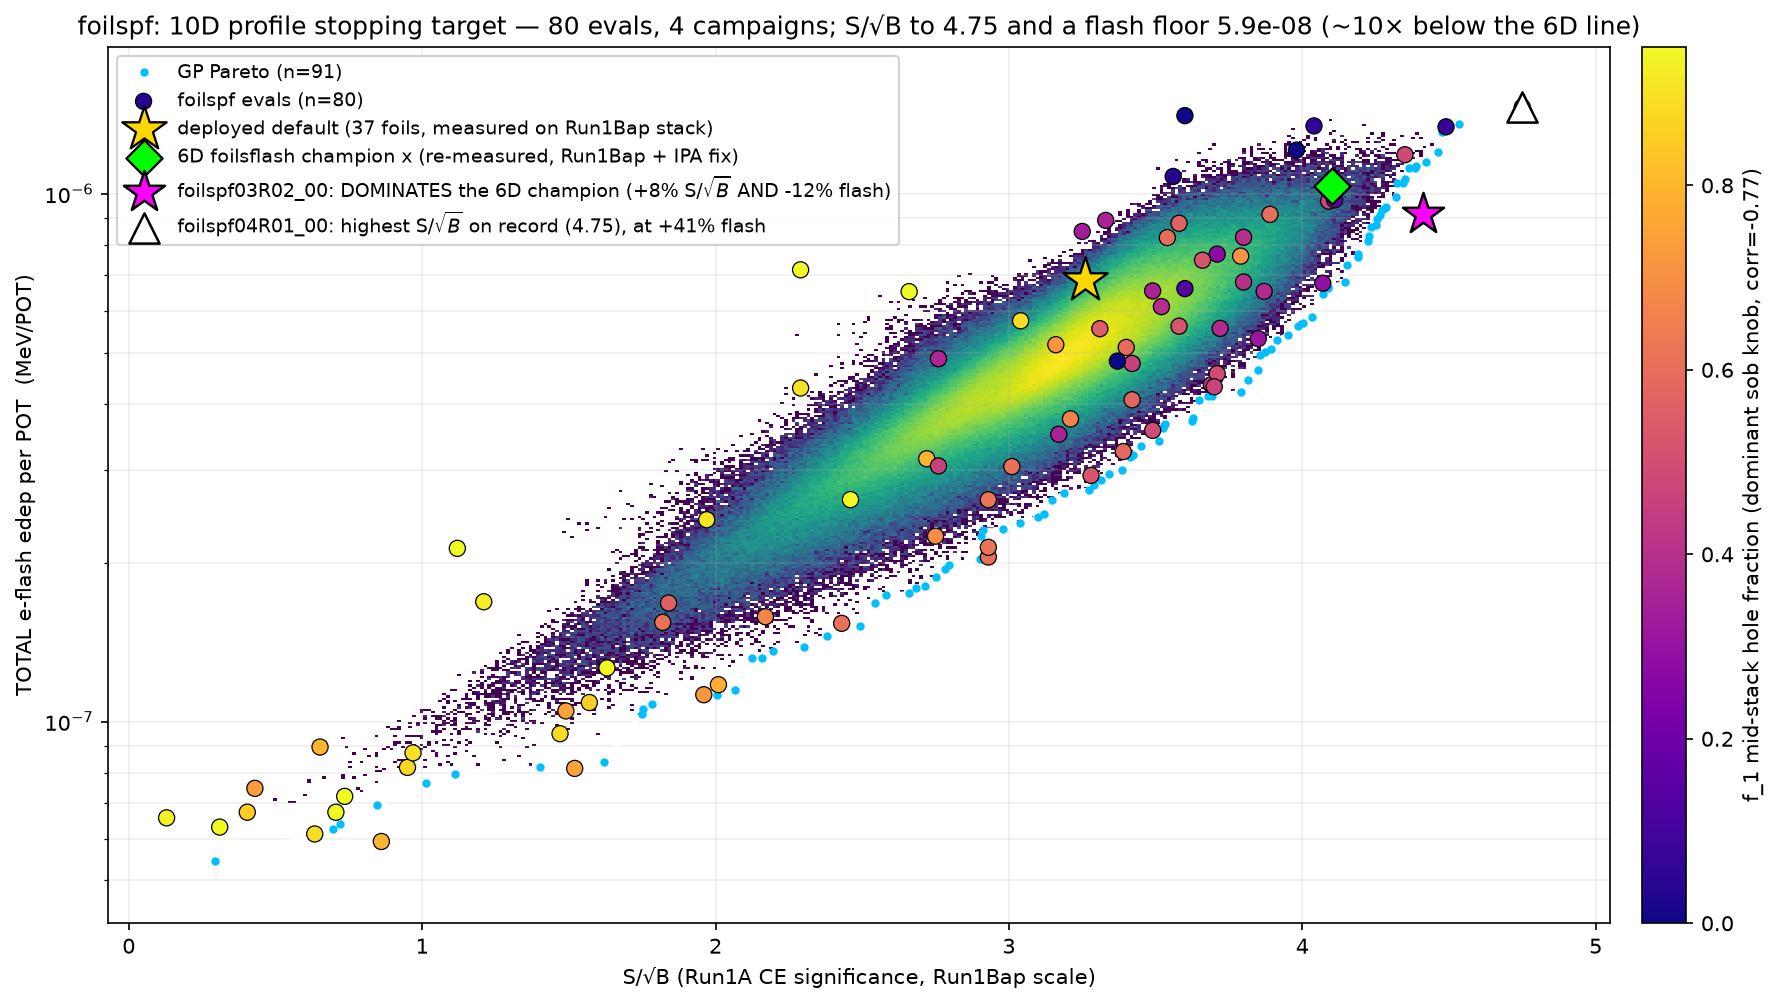
\includegraphics[height=0.72\textheight]{foilspf_perpot_cloud.png}
\end{center}
\footnotesize
80 evaluations, GP cloud over the 10D box. Gold star $=$ deployed default; green
diamond $=$ 6D champion geometry re-measured on this stack; \textbf{magenta star} $=$
\texttt{foilspf03R02\_00}, below and to the right of the diamond --- strictly better.
Colour $=$ mid-stack hole fraction, still the dominant S/$\sqrt{B}$ knob
(corr $-0.77$ at $n{=}80$): open mid holes shed stopping mass.
\end{frame}

\begin{frame}{Anatomy of the best point}
\begin{columns}
\begin{column}{0.55\textwidth}
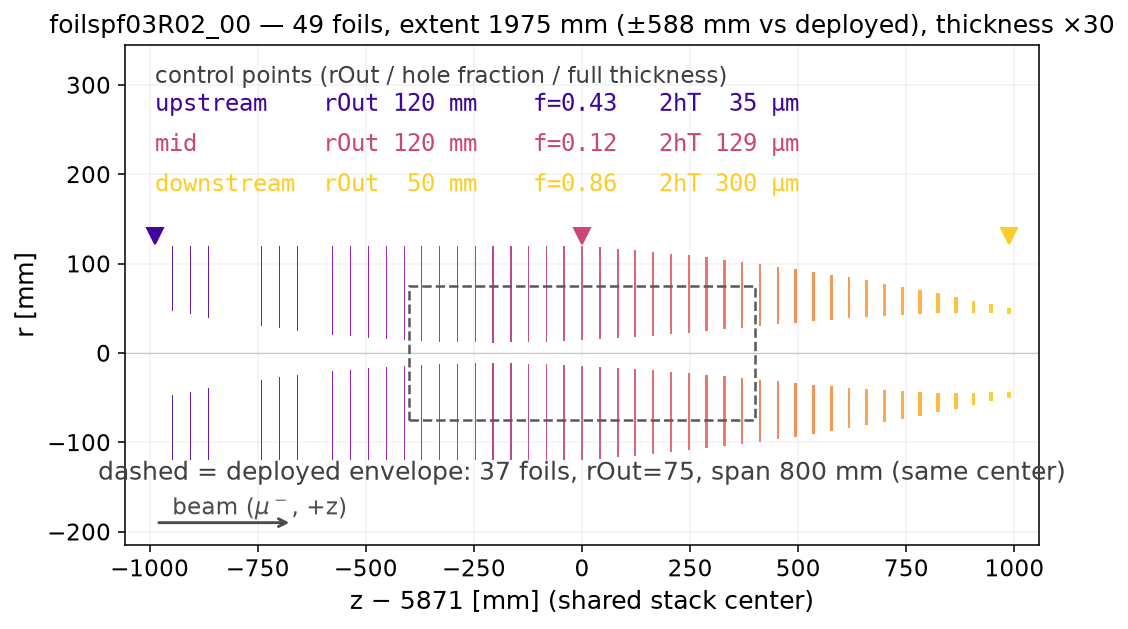
\includegraphics[width=\textwidth]{foilspf_bestsob_sketch.png}
\end{column}
\begin{column}{0.45\textwidth}
\small
\begin{tabular}{lcc}
\toprule
design & S/$\sqrt{B}$ & flash \\
\midrule
\texttt{03R02\_00} (champion)  & \textbf{4.41} & 0.92 \\
\texttt{04R01\_00} (max S/$\sqrt{B}$) & 4.75 & 1.46 \\
\texttt{04R03\_00} (flash-matched)    & 4.07 & 0.68 \\
6D champion $x$ (re-meas.)     & 4.10 & 1.04 \\
deployed default               & 3.26 & 0.69 \\
\texttt{02R02\_00} (flash floor) & 0.86 & \textbf{0.059} \\
\bottomrule
\end{tabular}
\vspace{0.4em}

{\scriptsize flash in $10^{-6}$ MeV/POT, all measured on the Run1Bap stack}
\vspace{0.6em}
\begin{itemize}\footnotesize
  \item Wide, nearly-solid discs (\texttt{rOut}~120~mm, $f{\to}0.12$) through the
        upstream half; tapering to \textbf{small thick annuli} downstream
        (\texttt{rOut}~50~mm, $f{=}0.86$, 300~µm).
  \item Extent 1975~mm --- $\pm$588~mm past the deployed span, growth
        \textbf{symmetric} about the shared center ($z_0{=}5871$), dashed $=$
        deployed envelope.
  \item Shape flipped vs the earlier 1015~mm champion, which put its mass
        \emph{downstream}. Mass-forward wins once the stack is long.
\end{itemize}
\end{column}
\end{columns}
\end{frame}

\begin{frame}{The extent knob --- and what we do \emph{not} know}
\begin{columns}[T]
\begin{column}{0.52\textwidth}
\small\textbf{What raising the ceiling bought}
\begin{itemize}\small
  \item \texttt{foilspf02} pinned the old 1100~mm bound: its two best new front
        points both sat \textbf{exactly on it}.
  \item Ceiling re-measured by live worst-corner preflight:
        1400, 1700 pass; 1800 fails. Moving one \textbf{massless} bookkeeping
        volume (\texttt{EMC\_Source}, a 20~µm vacuum disc no stage reads)
        reopened 1900 and 2000; 2100 fails.
  \item Rule adopted: extend only by relocating \textbf{massless} volumes,
        \textbf{never} real material.
  \item Split of the S/$\sqrt{B}$ gain: $+0.32$ from the higher bound,
        $+0.34$ from more search. Roughly half each.
\end{itemize}
\end{column}
\begin{column}{0.46\textwidth}
\small\textbf{Why longer helps}
\begin{itemize}\small
  \item Extent is \textbf{orthogonal to material by construction}: each foil's
        radius, thickness and hole are functions of its \emph{index} $i/48$, never
        of $z$. Extent sets only the pitch $\Delta z={}$extent$/48$ (8.3~mm at 400,
        41.7~mm at 2000; deployed 22.2~mm) --- a longer stack is the \emph{same
        foils spread further apart} (champion: 183~cm$^3$ at any length).
  \item The gain is therefore in \textbf{stopping} (corr $+0.35$); acceptance
        \emph{per stop} actually falls (corr $-0.37$). A longer stack intercepts
        more of the muon beam's range spread.
\end{itemize}
\vspace{0.3em}
\begin{alertblock}{\small Open --- no turnover observed}
\scriptsize
15 of 80 rows sit at \emph{exactly} 2000: the optimizer is still pushing at the
wall. 2000 is where the \textbf{zero-overlap corridor} ends, not where the physics
turns over --- \textbf{no proof it is optimal}. A fixed-shape scan would settle it.
\end{alertblock}
\end{column}
\end{columns}
\end{frame}

\begin{frame}{Machinery (unchanged)}
\begin{columns}[T]
\begin{column}{0.36\textwidth}
\centering
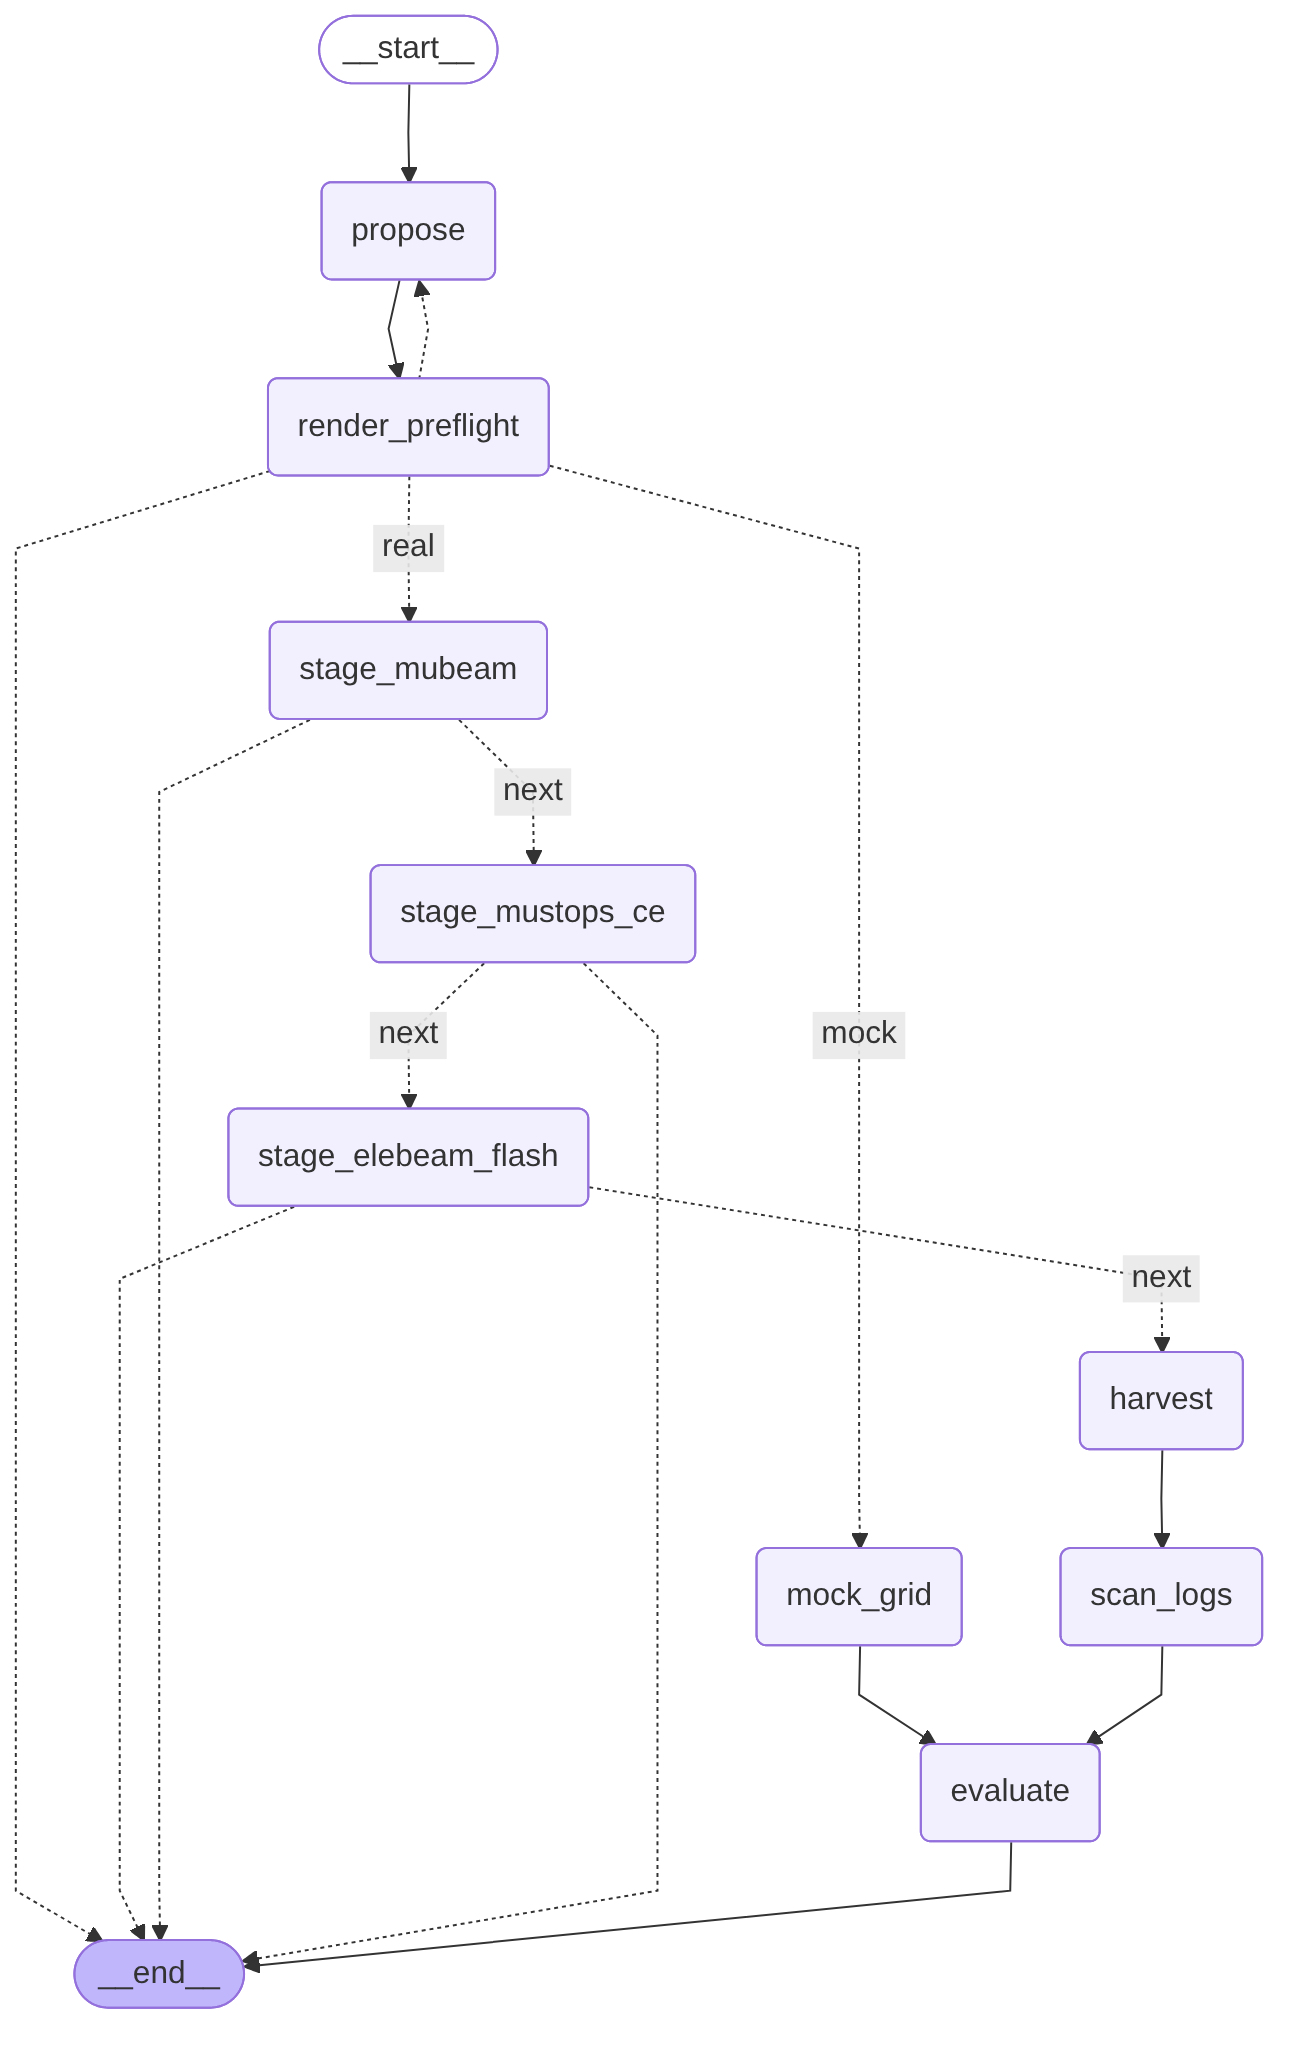
\includegraphics[height=0.78\textheight]{foilspf_langgraph.png}
\end{column}
\begin{column}{0.60\textwidth}
\small
Same closed loop as the 6D line --- generated from the running code
(\texttt{draw\_mermaid()}, foilspf mode):
\vspace{0.5em}
\begin{itemize}\small
  \item One LangGraph run $=$ one evaluation: propose $\rightarrow$ preflight
        $\rightarrow$ 3 grid stages $\rightarrow$ harvest $\rightarrow$ row.
  \item \texttt{hybrid} picker (qNEHVI $+$ qNParEGO), $q{=}10$ in flight, rolling
        to 20 evals per campaign; GP refits as rows land.
  \item Preflight \textbf{requires zero overlaps} --- reachable only on this
        corrected stack.
  \item No row is ever written from partial results: 80 launched, 80 landed.
\end{itemize}
\vspace{0.5em}
{\tiny
\texttt{python -m graph.closed\_loop --mode foilspf \textbackslash}\\
\texttt{\ \ --picker hybrid --q 10 --rolling --max-evals 20}
}
\end{column}
\end{columns}
\end{frame}

\begin{frame}{Conclusion \& next steps}
\begin{itemize}
  \item The profile parameterization is \textbf{strictly stronger} than the 6D
        extras --- not merely competitive: it wins on S/$\sqrt{B}$ \emph{and} flash
        simultaneously, and reaches a flash floor $\sim$10$\times$ lower.
  \vspace{0.4em}
  \item The most deployable point may not be the champion:
        \texttt{foilspf04R03\_00} offers \textbf{$+25\%$ S/$\sqrt{B}$ over the
        deployed target at the deployed target's own flash}.
  \vspace{0.4em}
  \item Still on \textbf{clean geometry}: correct absorber position, zero
        overlaps --- no 6D row can claim either.
  \vspace{0.4em}
  \item \textbf{Running now:} \texttt{foilspf2k01} --- 9D \emph{shape-only} at extent
        pinned to 2000, to ask how much is left in shape once length is fixed.
  \vspace{0.4em}
  \item \textbf{Needed:} a controlled extent scan at fixed shape (400\ldots2400) to
        find the actual optimum --- the geometry corridor reaches $\sim$2400 if the
        stack is also shifted upstream. And a 400-job flash confirmation of
        \texttt{foilspf03R02\_00}.
\end{itemize}
\end{frame}

\end{document}
